\section{Experiments}
Our experiments are about two main tasks: binary and multi-class classification. In this section, first we describe the dataset and the variations created to perform sensitivity analysis. Then, we go trough the experiments setup where we describe how we have conducted the experiments to accomplish the two tasks and finally we show the results.
\subsection{Datasets}
\begin{figure}
	\begin{center}
		\fbox{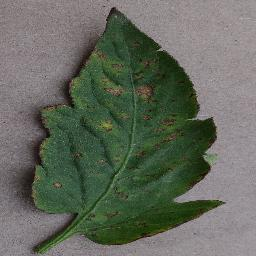
\includegraphics[scale=0.167]{./images/normal_3159}
			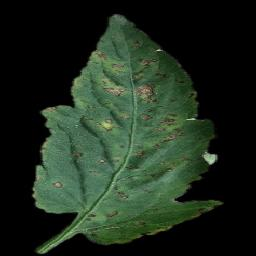
\includegraphics[scale=0.167]{./images/segmented_3159}
			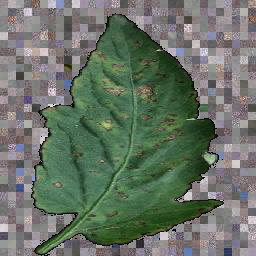
\includegraphics[scale=0.2241]{./images/9_ROTATE_180_crop}
			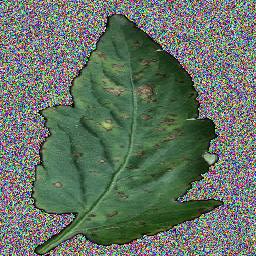
\includegraphics[scale=0.167]{./images/196_ROTATE_270}
			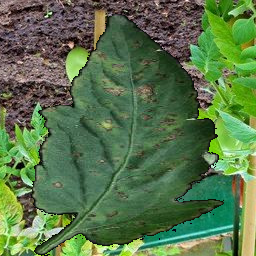
\includegraphics[scale=0.2241]{./images/random_backgorund}
		}
		\begin{center}
			\caption{\textit{Samples of dataset images, from left to right: \textbf{Original}, \textbf{Segmented}, \textbf{Random Background Crop}, \textbf{Random Noise Background} and \textbf{Random Background Image}.}}
			\label{fig:samples}
		\end{center}
		\vspace{-32pt}
	\end{center}
\end{figure}
We analyze 18,158 images of tomato plant leaves, which are split in 10 classes, 9 diseases and 1 healthy. The scope is to predict the correct class of a leaf image. All the images are RGB and sized 256x256 pixels.
The classes are: (A) Bacterial Spot $2,127$ samples, (B) Early Blight $1,000$ samples, (C) Late Blight $1,909$ samples, (D) Leaf Mold  $952$ samples, (E) Septoria Leaf Spot $1,771$ samples, (F) Two-spotted Spider Mites $1,676$ samples, (G) Target Spot $1,404$ samples, (H) Tomato Yellow Leaf Curl Virus $5,356$ samples, (I) Tomato Mosaic Virus $373$ samples, (J) Healthy $1,590$ samples.
\\\indent
Given the original dataset we conduct the training phase on different variations of the original dataset, we work on the backgrounds in order to find a way to overcome the limits highlighted in \cite{ref33, ref10} and confirmed by us. Especially, we have found out a dependence between the original backgrounds and their belonging class.
In Figure \ref{fig:samples} we can see all the images and the different variations of the dataset we have tested.
\begin{itemize}
	\vspace{-5pt}
	\item{\textbf{Original dataset.} It consists of images of tomato leaves laying over a gray table.}
	\vspace{-5pt}
	\item{\textbf{Segmented dataset.} It consists of images of tomato leaves with no background, this variation has been used also in \cite{ref10}. In our work we have re-segmented the images since in the available segmented dataset they were incomplete.}
	\vspace{-5pt}
	\item{\textbf{Random Background Crop dataset.} It consists of the leaf images coming from PlantVillage with a background composed of crops of background coming from the Original dataset.}
	\vspace{-5pt}
	\item{\textbf{Random Noise Background dataset.} It consists of leaf images coming from PlantVillage with a background composed of random colored pixels.}
	\vspace{-5pt}
	\item{\textbf{Random Background Image dataset.} It consists of leaf images coming from PlantVillage dataset, each with a background taken from a set of 4,176 images we have built by looking for tomato plantation pictures on the Internet. The objective of this dataset is not only to decouple the background influence on the classifier but also to try to bring the leaf to a realistic situation, where the leaf image is taken directly from the plantation.}
\end{itemize}
\subsection{Experiments setup}
\begin{figure}
	\begin{center}
		\fbox{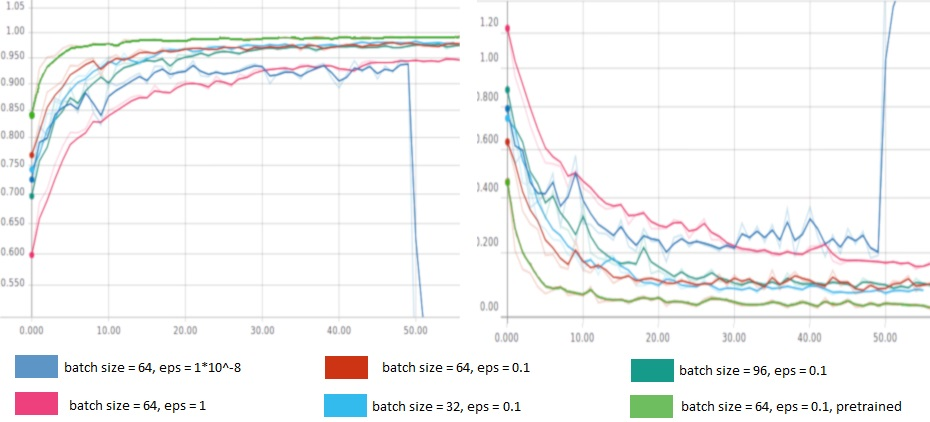
\includegraphics[scale=1.3]{./images/tensorboards}}
		\begin{center}
			\caption{\textit{Validation accuracy over epochs}.}
			\label{fig:tensorboard}
		\end{center}
		\vspace{-40pt}
	\end{center}
\end{figure}
\subsubsection{Data augmentation and normalization}
We perform data augmentation applying to each original sample two randomly selected transformations from this pool: Flip Top Bottom, Flip Left Right, Rotate 90\degree, Rotate 180\degree, Rotate 270\degree, Flip Top Bottom and Rotate 90\degree, Flip Top Bottom and Rotate 270\degree.
\\
Another key aspect of our setup is the normalization of the input images, indeed, the chosen normalization changes dramatically the model performance. In our work we consider the following normalization approaches:
\\
\textbf{Dataset Normalization.} Given the chosen variation of the dataset we compute the mean and the standard deviation of the train dataset.
\\
\textbf{Per-leaf Normalization.} Starting from the segmented train dataset we compute the mean and standard deviation of the non-black pixels. \vspace{-10pt}
\subsubsection{Binary classification setup}
\textbf{LeNet architecture.} This network, proposed in \cite{ref30}, is the first and simplest deep model available. We have adapted the first and the last convolutional layers to fit our images size and the last fully connected layer to perform our binary task.
\\
\textbf{Weights initialization.} For this network we start by using training from scratch approach. The weights in the network are initialized using Xavier initialization \cite{ref31}. This helps the training since we start from a normally distributed set of weights and we avoid that certain weighs vanish through epochs.
\\
\textbf{Activation function.}
The layers activation function is the rectified linear unit (ReLU) function since it diminishes the likelihood of a gradient to vanish.
\\
\textbf{Loss function.}
The chosen loss function for the binary classification is the binary cross-entropy since it is properly designed for binary tasks.
\\
\textbf{Optimizer.}
We have chosen Adam with its default parameters. It is based on adaptive estimates of lower-order moments and it is computationally efficient.
\\
\textbf{Validation.}
For this task we perform 10-fold cross validation. This kind of validation is used to estimate the model performance and therefore to select the hyper-parameters.
\subsubsection{Multi-class classification setup}
\textbf{AlexNet architecture.}
For this task we choose a more complex model since we have first tested LeNet architecture achieving results far from the state-of-the-art \cite{ref11}.
\\
\textbf{Weights initialization.}
For this network we try both training from scratch approach and transfer learning. The weights in the first case are initialized using Xavier initialization (\cite{ref31}). In the transfer learning approach, instead, we use the weights coming from the training on ImageNet \cite{imagenet}.
\\
\textbf{Activation function.}
Layers activation function is the rectified linear unit (ReLU) function.
\\
\textbf{Loss function.}
In this case we use cross-entropy as loss function since it is largely used for multi-class classification tasks.
\\
\textbf{Optimizer.}
As optimizer we have chosen Adam \cite{ref32}. An important annotation should be done about this optimizer. Indeed, through the training process we have noticed that the accuracy after a certain number of epochs largely drops as we can see in Figure \ref{fig:tensorboard}. This has been caused by the $\varepsilon$ parameter. It is used to avoid division by zero when the gradient is almost zero during Adam parameters update. By default it is set to $10^{-8}$, however in some cases it causes large network weights updates. Therefore, we set it to $0.1$ in order to avoid this problem. All the other parameters are set to their default values.
\\
\textbf{Validation.}
In the case of multi-class classification we opt to proceed with cross-validation. We have chosen a different approach from binary classification. Indeed, k-fold cross validation applied to AlexNet requires massive computational time that is not justified since we have checked that there is a small amount of variance across different validation folds.
\subsection{Results and discussion}
\subsubsection{Binary classification}
We set up a binary dataset composed of two classes: healthy (J) and infected (A, B, C, D, E, F, G, H, I). After a training phase using 10-fold cross-validation, we select as best hyper-parameters for our binary classification problem, the batch size equal to $32$ and the total number of epochs equal to $15$. With this configuration, after re-training the model on the whole train set, we obtain an average accuracy of $99.92\%$. As expected we obtained the healthy class accuracy lower than the infected one because, since the dataset is unbalanced, the model sees more infected samples. As a further analysis, we have to consider that for our unbalanced dataset the baseline accuracy is $90\%$, therefore just looking at the accuracy is not enough in this case. The F1-score ($99.50\%$) can better assess the performance of the model, which are satisfactory.
\begin{table}
	\centering
	\begin{center}
		\footnotesize
		\begin{tabular}{|c|c|c|}
			\hline
			Train & Test & Performance\\ 
			\hline
			\multirow{4}*{Original}
			& Original & 
			\begin{tabular}{@{}c@{}}
				$Average Accuracy = \textbf{0.99856} $ \\
				$Precision_{M} = \textbf{0.99834} $ \\
				$Recall_{M} = \textbf{0.99817} $ \\
				$F_{1} score_{M} = \textbf{0.99825} $ \\
			\end{tabular} \\
			\cline{2-3}
			& Segmented &
			\begin{tabular}{@{}c@{}}
				$Average Accuracy = 0.39017$ \\
				$Precision_M = NaN$ \\
				$Recall_M = 0.28588$ \\
				$F_1 score_M = NaN$ \\
			\end{tabular} \\  				
			\hline
			\multirow{4}*{Segmented}
			& Original & 
			\begin{tabular}{@{}c@{}}
				$Average Accuracy = 0.61793$ \\
				$Precision_M = 0.73020$ \\
				$Recall_M = 0.49413$ \\
				$F_1 score_M = 0.48694$ \\
			\end{tabular} \\
			\cline{2-3}
			& Segmented &
			\begin{tabular}{@{}c@{}}
				$Average Accuracy = 0.96651$ \\
				$Precision_M = 0.95952$ \\
				$Recall_M = 0.95689$ \\
				$F_1 score_M = 0.95802$ \\
			\end{tabular} \\  				
			\hline
			\multirow{6}*{\shortstack[1]{Random\\ Background \\Crop}}
			& Original & 
			\begin{tabular}{@{}c@{}}
				$Average Accuracy = 0.76918$ \\
				$Precision_M = 0.79434$ \\
				$Recall_M = 0.673089$ \\
				$F_1 score_M = 0.67152$ \\
			\end{tabular} \\
			\cline{2-3}
			& Segmented &
			\begin{tabular}{@{}c@{}}
				$Average Accuracy = 0.84804$ \\
				$Precision_M = 0.88554$ \\
				$Recall_M = 0.73743$ \\
				$F_1 score_M = 0.73997$ \\
			\end{tabular} \\  				
			\hline
			\multirow{6}*{\shortstack[1]{Random\\ Noise \\Background}}
			& Original & 
			\begin{tabular}{@{}c@{}}
				$Average Accuracy = 0.57886$ \\
				$Precision_M = 0.66675$ \\
				$Recall_M = 0.49010$ \\
				$F_1 score_M = 0.49930$ \\
			\end{tabular} \\
			\cline{2-3}
			& Segmented &
			\begin{tabular}{@{}c@{}}
				$Average Accuracy = 0.74847$ \\
				$Precision_M = 0.82094$ \\
				$Recall_M = 0.70987$ \\
				$F_1 score_M = 0.69742$ \\
			\end{tabular} \\  								
			\hline
			\multirow{6}*{\shortstack[1]{Random\\ Background\\ Images}}
			& Original & 
			\begin{tabular}{@{}c@{}}
				$Average Accuracy = \textbf{0.93230}$ \\
				$Precision_{M} = \textbf{0.92596}$ \\
				$Recall_{M} = \textbf{0.91333}$ \\
				$F_{1} score_{M} = \textbf{0.91639}$ \\
			\end{tabular} \\
			\cline{2-3}
			& Segmented &
			\begin{tabular}{@{}c@{}}
				$Average Accuracy = \textbf{0.94977}$ \\
				$Precision_{M} = \textbf{0.94297}$ \\
				$Recall_{M} = \textbf{0.92846}$ \\
				$F_{1} score_{M} = \textbf{0.93450}$ \\
			\end{tabular} \\  				
			\hline
		\end{tabular}
	\end{center}
	\caption{\textit{Performance of multi-class classification. $NaN$ identifies the presence of never predicted classes.}}
	\label{table:sensitivity}
	\vspace{-14pt}
\end{table}
\subsubsection{Multi-class classification}
As we have done for binary classification, we try several configurations by using different hyper-parameters and we test our results on the validation set. As figure \ref{fig:tensorboard} shows, the best configuration found is AlexNet pre-trained, with batch size equal to 64, $\varepsilon$ equal to 0.1 trained for 57 epochs. We have also tried some configurations using weight decay regularization and changing the initial learning rate. The resulting performances were not as good as the one on the chosen configuration. We think that weight decay did not help to improve performances because we have a fairly large dataset and AlexNet is not enough complex to reach overfitting. Furthermore, in AlexNet there are dropout layers that limit this problem. For what concerns the learning rate, Adam optimizer \cite{ref32} automatically adapts it after some epochs. Hence, most of the job is done by the optimizer and our selected learning rates involves the first few epochs of training and not the overall training.
\\
The results obtained in the chosen configuration are shown in the first row of Table \ref{table:sensitivity}. AlexNet pre-trained has a very good performance in all the classes and has obtained also better results than the state-of-the-art \cite{ref11}. We expected that classes with less samples, e.g. (I) Tomato Mosaic Virus, would have been wrongly classified compared to classes with an higher number of samples, e.g. (H) Tomato Yellow Leaf Curl. This is not our case, since our classifier wrongly classifies only some samples that are not related to the size of the predicted class. ===additional material conf matrix?===
\vspace{-8pt}
\subsubsection{Sensitivity analysis}
After a good level of accuracy for our multi-class classification task has been reached, we move our attention to the analysis of robustness of our classifier trained on the Original dataset. Hence, we test the model against the Segmented dataset. In particular, in Table \ref{table:sensitivity} we can notice that the accuracy drops and some classes are never predicted causing Precision and F1-score to have $NaN$ value. From this result and from visualization methods we deduced that the model somehow learned patterns in the background. Table \ref{table:sensitivity} describes all the different settings we have tried and the related results. For each approach, we test the model against both Normal and Segmented dataset using Dataset Normalization. First, we use the Segmented dataset for the training phase. Also in this case the trained model has not been able to satisfactorily identify the leaves when tested against the Normal dataset. We have obtained better results using Random Background Crop and Random Noise Background datasets. As final result, we propose the usage of Random Background Images dataset. In this case we use Per-leaf Normalization in order to further make each leaf image independent from its background. The results are shown in Figure \ref{fig:conf_matrix}. This model is the only with an high value on precision and recall, sign of robustness. It is possible to see in Figure \ref{fig:gradcam} the differences on the activation of GradCAM: the first is the outcome of our first model and the activations are distributed both on the leaf and on the background, the latter is the outcome of our chosen model and the activations are located only on the leaf.
\begin{figure}[t]
	\begin{center}
		\fbox{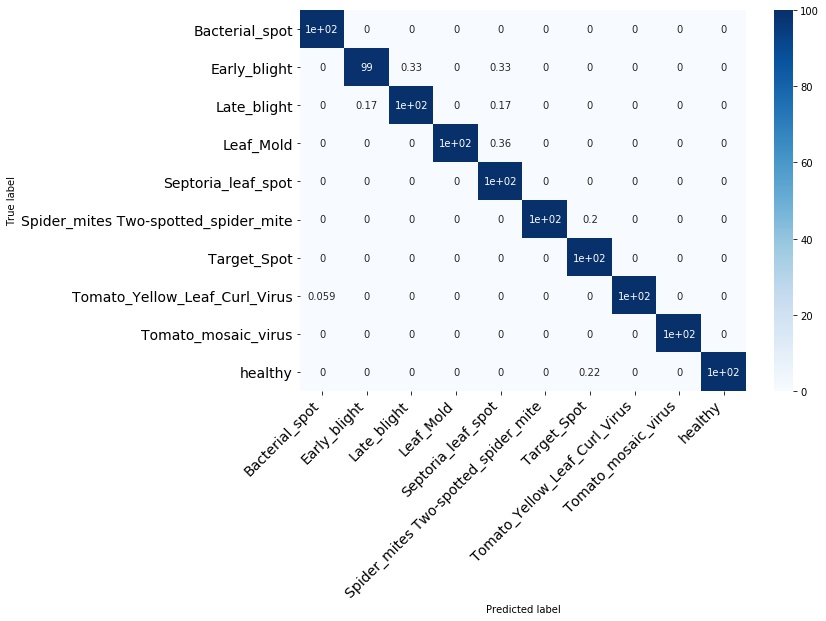
\includegraphics[scale=0.5]{./images/conf_matrix_norm}}
	\end{center}
	\caption{\textit{Confusion matrix of AlexNet pretrained in multi-class classification problem in percentage using per-leaf normalization and random background images.}}
	\label{fig:conf_matrix}
	\label{fig:long}
	\label{fig:onecol}
	\vspace{-5pt}
\end{figure}
\begin{figure}
	\begin{center}
		\fbox{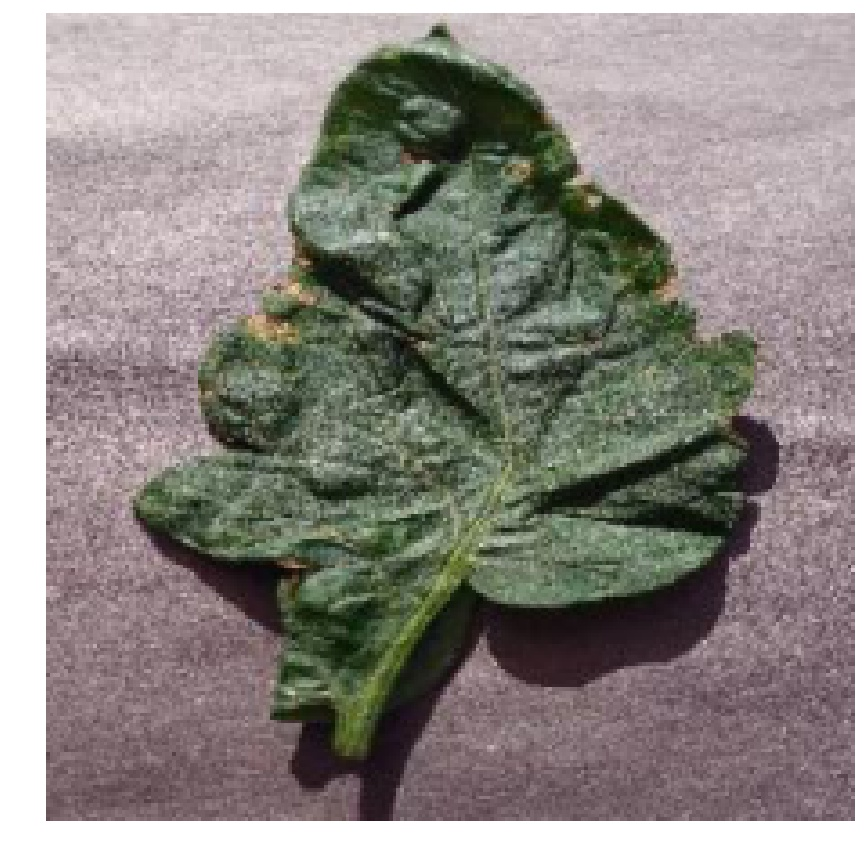
\includegraphics[scale=0.11]{./images/Target_Spot2_orig}
			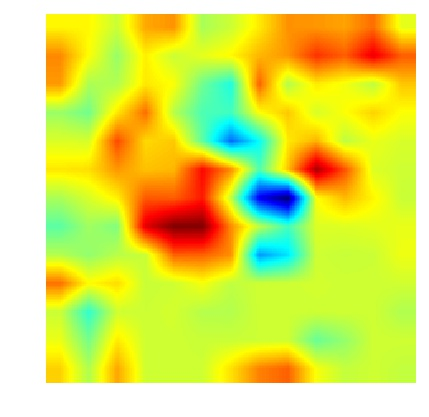
\includegraphics[scale=0.24]{./images/Target_Spot2_cam}
			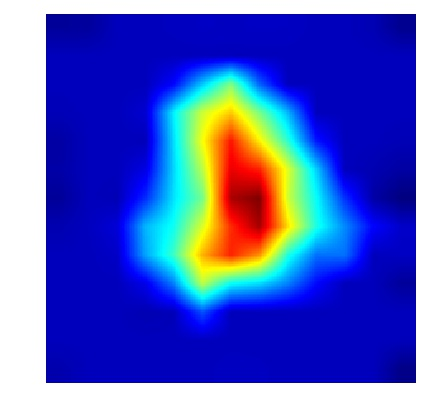
\includegraphics[scale=0.24]{./images/Target_Spot2normal_cam}
		}
	\end{center}
	\caption{\textit{From left to right: Original image, class: Target Spot, GradCAM on Original dataset, GradCAM on Random Background Image.}}
	\label{fig:gradcam}
	\label{fig:long}
	\label{fig:onecol}
	\vspace{-15pt}
\end{figure}